\documentclass[11pt]{article}
\usepackage[T1]{fontenc}
\usepackage{lmodern}
\usepackage[margin=1in]{geometry}
\usepackage{microtype,booktabs,tabularx,amsmath,graphicx,enumitem,caption}
\usepackage[dvipsnames]{xcolor}
\usepackage[colorlinks=true,linkcolor=MidnightBlue,urlcolor=MidnightBlue,citecolor=MidnightBlue]{hyperref}
\usepackage{titlesec}
\titleformat{\section}{\large\bfseries}{\thesection}{0.6em}{}
\titleformat{\subsection}{\normalsize\bfseries}{\thesubsection}{0.6em}{}
\captionsetup{font=small,labelfont=bf}
\setlist{itemsep=2pt,topsep=4pt}
\newcommand{\dBmHz}{\,dBm/Hz}
\newcommand{\draftnote}[1]{\textcolor{BrickRed}{\textit{[#1]}}}

\title{Reducing receiver noise on the UAV-RT tracking drone\\[4pt]
\large Test report --- draft 0.1}
\author{Michael W.\ Shafer, Northern Arizona University\\
\small Analysis and drafting assisted by Claude (Anthropic)}
\date{19 November 2026}

\begin{document}
\maketitle

\noindent\fbox{\parbox{\dimexpr\linewidth-2\fboxsep-2\fboxrule}{\small
\textbf{Draft.} This report covers the tests run up to 18 November 2026. Two further tests are
planned and will be added: a same-day flight comparison of the Airspy Mini and Airspy HF+, and a
reference measurement of the site's background noise with the antenna raised on a mast and the drone
switched off (Section~\ref{sec:next}). Numbers that those tests may change are marked in the text.}}

\section{Summary}

The tracking drone receives very-high-frequency (VHF) radio pulses from wildlife tags near
160~MHz. During the March 2025 fieldwork on Ponui Island, the receiver's background noise rose by
16--17~dB whenever the drone flew. Between then and November 2026 the receiver, its antenna feed and
the drone's wiring were changed to reduce that noise. This report measures the result.

\begin{itemize}
\item \textbf{The noise reaching the receiver in flight fell by about 18~dB}: from about
$-145$\dBmHz{} at Ponui to $-163.5$\dBmHz{} on 14 November 2026 (Figure~\ref{fig:dumbbell}).
The two figures were measured with different receivers at different sites; a signal-generator
calibration of both receivers (Section~\ref{sec:bench}) puts them in the same units.
\item \textbf{In flight, the noise is now only 3.3~dB above the receiver's own internal noise.}
At Ponui it was 22~dB above. Further reductions on the aircraft can gain at most 3.3~dB, and part of
that is likely the antenna hearing ordinary background noise from the surroundings
(Section~\ref{sec:budget}).
\item \textbf{The common-mode choke on the antenna coax and the 15~ft coax extension do most of the
work in flight.} Without either, the in-flight noise was 10~dB above the receiver's own noise; with
both, 3.3~dB (Table~\ref{tab:flights}).
\item \textbf{The two receivers are about equally sensitive}: noise figures of 6.3--6.4~dB for the
Airspy Mini and 7.2~dB for the Airspy HF+, as installed. \textbf{The HF+ handles strong signals far
better}: a $-90$~dBm tone raised the Mini's noise near it by 14~dB and left the HF+ unchanged
(Figure~\ref{fig:desense}).
\end{itemize}

\begin{figure}[!htbp]
\centering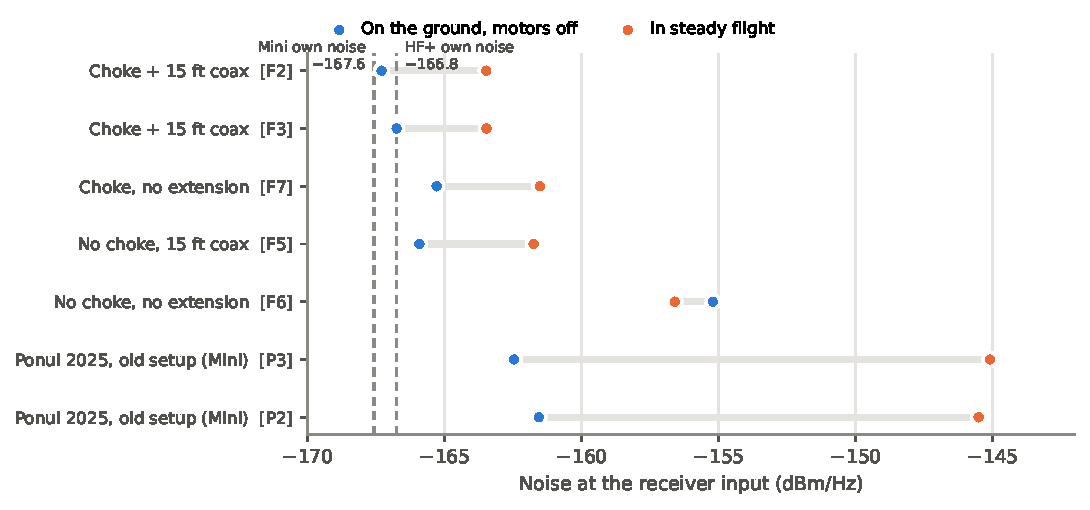
\includegraphics[width=\linewidth]{figures/fig1_dumbbell.pdf}
\caption{Noise at the receiver input, on the ground with the motors off (blue) and in steady flight
(orange), for each configuration. Dashed lines: each receiver's own internal noise, measured on a
50~$\Omega$ load. F2--F7 are the 14 November 2026 flights; P2 and P3 are Ponui flights from March 2025.}
\label{fig:dumbbell}
\end{figure}

\section{Background}

\subsection{Why the noise matters}
The detector looks for the tag's 20~ms pulses against the background noise in a 3.8~kHz-wide
channel around the tag's frequency. Every decibel of extra background noise is a decibel of lost
signal-to-noise ratio, which shortens the distance at which a tag can be detected. A rise of
16--17~dB in flight, as at Ponui, cuts the free-space detection range by a factor of about seven.

\subsection{What changed between Ponui and now}
At Ponui the receiver was an Airspy Mini on a USB extension from the onboard Raspberry Pi, feeding
an omnidirectional antenna hanging about 15~ft (4.6~m) below the drone on RG-316 coax, with no
ferrites and no shielding. Since then:
\begin{itemize}
\item the receiver is an Airspy HF+ Discovery;
\item a common-mode choke --- 12 turns of the coax, as a crossover winding, on a Fair-Rite
5943002701 mix-43 toroid --- sits at the receiver's antenna input;
\item the fuselage and arms are covered by an RF-shielding fabric, with the USB cable passing
through a bulkhead bonded to the shield;
\item mix-43 ferrite cores are fitted on the battery, motor-controller, regulator, radio-link, CAN
and GPS cables;
\item the 5~V regulator and the battery monitor are individually wrapped and grounded.
\end{itemize}
The full design, with the reasoning for each change, is in \texttt{hardware/emi-design.md} of the
UAV-RT hub repository. None of the individual ferrites has yet been measured on its own.

\subsection{Terms used}
\begin{description}[leftmargin=1.2em,style=nextline]
\item[Noise floor] The background noise power per hertz of bandwidth in the detector's channel,
with no tag signal present. Reported in dBm/Hz (decibels relative to one milliwatt, per hertz).
\item[Receiver's own noise] The noise floor with a 50~$\Omega$ load in place of the antenna: what
the receiver produces by itself. Any noise above this level comes in from outside.
\item[Noise figure (NF)] How much noise the receiver adds, in dB, relative to the unavoidable
thermal noise of a resistor at room temperature ($kT_0 = -174$\dBmHz).
\item[Common-mode current] Noise current flowing on the outside of a cable's shield, or on all
its wires together. Ferrite chokes block it.
\item[Receiver units] Each receiver's software reports power in its own arbitrary digital units.
The two receivers' units differ by 35.7~dB; Section~\ref{sec:compare} shows how one converts to
the other, and the calibration in Section~\ref{sec:bench} converts both to dBm.
\end{description}

\section{Test configurations}

\begin{table}[!htbp]
\centering\small
\begin{tabularx}{\linewidth}{@{}l l X l@{}}
\toprule
Test & Date & Configuration & Receiver \\
\midrule
P2, P3 & 2025-03-22 & Ponui flights; old setup: 15~ft coax, no choke, no ferrites or shielding & Mini, gain 20 \\
F2, F3 & 2026-11-14 & Choke + 15~ft coax; climb to $\sim$170~ft, F2 with a 30~s hover & HF+ \\
F5 & 2026-11-14 & No choke, 15~ft coax; 50~ft & HF+ \\
F6 & 2026-11-14 & No choke, no coax extension; 50~ft & HF+ \\
F7 & 2026-11-14 & Choke, no coax extension; 50~ft & HF+ \\
VNA & 2026-11-17 & Insertion and return loss of the coax, choke and bench cable & --- \\
Bench & 2026-11-18 & Signal generator into each receiver on the drone's Pi, motors off & Mini (gain 21), HF+ \\
\bottomrule
\end{tabularx}
\caption{Tests in this report. All flights and bench runs were at 160.172~MHz, the frequency of the
last Ponui flight. No tag was transmitting during the 2026 flights.}
\label{tab:tests}
\end{table}

\noindent The flights on 14 November had no telemetry recorded for the radio flights, so the stages
of each flight --- motors off on the ground, takeoff, steady flight, landing --- were read from the
noise itself and from the flight notes. The PX4 flight logs from the flight controller will
replace these estimates when added.

\section{Methods}
\label{sec:methods}

\subsection{Recordings}
Every test used the drone's own receive chain, the same software that runs in flight. The
controller on the Raspberry Pi tunes the receiver, reduces the sample rate to one narrow channel
around the tag frequency, and passes it to the detector, which writes the raw samples to a file
(\texttt{data\_record.<id>.1.bin}: complex 32-bit floating-point samples, no timestamps).
\begin{itemize}
\item Airspy Mini: sampled at 3~MS/s, decimated by 8 and channelized to 3750~samples/s.
\item Airspy HF+: sampled at 768~kS/s, tuned 10~kHz high and shifted back, decimated by 200 to
3840~samples/s.
\end{itemize}

\subsection{Noise floor from a recording}
Each second of samples is cut into $M$ blocks of $N=256$ samples. For block $m$, with a Hann window
$w[n]$ and sample rate $f_s$, the power spectral density is
\begin{equation}
P_m(f_k) = \frac{\left|\sum_{n=0}^{N-1} w[n]\,x_m[n]\,e^{-j2\pi kn/N}\right|^2}{f_s\sum_{n} w[n]^2}
\quad\text{(receiver units per Hz).}
\end{equation}
The noise floor for that second is the median over the $M$ blocks, then the median over the inner
80\% of the frequency bins:
\begin{equation}
\hat N = \operatorname*{median}_{k\,\in\,\text{inner }80\%}\;\operatorname*{median}_{m}\;P_m(f_k).
\end{equation}
The median over blocks removes tag pulses, which occupy 20~ms of each 1.33~s, so the Ponui
recordings, which contain pulses, give the background alone. The median of an exponentially
distributed power is $\ln 2$ times its mean, so $\hat N$ reads about 1.6~dB below the true mean
noise. That bias cancels in every conversion below, because the same estimator is applied to the
calibration recordings. Script: \texttt{tools/noise\_floor.py}.

\subsection{Calibration with a signal generator}
\label{sec:calmethod}
On the bench, an Agilent E4432B generator produced a steady tone at 160.1725~MHz (500~Hz inside the
channel) through an N-to-SMA adapter, 88~cm of RG-316 and the choke, into each receiver in turn.
Each run held, for one to two minutes each: a 50~$\Omega$ load on the receiver; the generator
connected with its output off; then the tone at $-120$, $-110$, $-100$ and $-90$~dBm. The order was
Mini, HF+, Mini.

The tone's power in the recording is the sum of the spectrum above the local noise over the bins
around the tone,
\begin{equation}
S = \sum_{k\in\text{tone}}\bigl(\bar P(f_k) - N_\text{local}\bigr)\,\Delta f ,
\end{equation}
where $\bar P$ is the mean spectrum over the step and $\Delta f = f_s/N$ is the bin width. The
receiver's gain from dBm at its input to its own units is then
\begin{equation}
G = 10\log_{10} S - \bigl(P_\text{gen} - L_\text{path}\bigr),
\end{equation}
with $P_\text{gen}$ the generator setting and $L_\text{path} = 0.6$~dB the measured loss of the cable
and choke (Section~\ref{sec:vna}). The receiver's own noise, referred to its input, and its noise
figure follow from the 50~$\Omega$ load step:
\begin{equation}
N_\text{in} = 10\log_{10} N_\text{load} - G \quad\text{(dBm/Hz)},\qquad
\text{NF} = N_\text{in} - 10\log_{10}\!\frac{k_B T}{1\,\text{mW}},
\end{equation}
with $k_B T = -173.9$\dBmHz{} for a load at about 295~K. Script:
\texttt{tools/bench\_calibration.py}.

\subsection{Converting the flight recordings to dBm/Hz}
A flight's noise floor $m_\text{flight}$, in receiver units, converts through the same receiver's
calibration-load reading $m_\text{load}$, taken with the same estimator, and that load's known
input-referred noise:
\begin{equation}
N_\text{flight} = N_\text{in,load} + \bigl(m_\text{flight} - m_\text{load}\bigr).
\end{equation}
This assumes the receiver ran at the same gain in flight as on the bench. That holds exactly for
the HF+, whose settings are fixed. The Mini ran at gain 20 at Ponui and 21 on the bench (the setting
TagTracker now uses and does not expose), so the Ponui values carry an uncertainty of the gain
difference between those two settings, likely 1--2~dB.

\subsection{Comparing Mini and HF+ readings directly}
\label{sec:compare}
The two receivers' software report power in different arbitrary units, so their raw readings cannot
be compared as they stand. The calibration gives each receiver's gain $G$ from dBm at its input to its
own units (Section~\ref{sec:calmethod}). The difference between the two gains converts one
receiver's units into the other's:
\begin{equation}
\Delta G = G_\text{Mini} - G_\text{HF+} = 59.86 - 24.11 = 35.7\ \text{dB},
\qquad
m_\text{HF+ units} = m_\text{Mini units} - \Delta G .
\end{equation}
A Mini reading is 35.7~dB higher than an HF+ reading of the same signal at the antenna input.
Three things make this valid:
\begin{itemize}
\item \textbf{Both readings are per hertz.} Each spectrum is divided by its own sample rate
($f_s$ in Equation~1), so the Mini's 3750~samples/s and the HF+'s 3840~samples/s do not matter.
\item \textbf{Both use the same estimator}, so its bias cancels. Measured on the 50~$\Omega$ load,
the bias was $-1.64$~dB for the Mini and $-1.68$~dB for the HF+, a difference of 0.04~dB.
\item \textbf{$\Delta G$ does not depend on the generator's absolute accuracy or on the 0.6~dB path
loss.} The same generator, cable and choke fed both receivers, so any error in them shifts both gains
equally and cancels in the difference. $\Delta G$ is therefore more certain than either gain alone.
\end{itemize}
It holds only at the gain settings calibrated: Mini gain 21, and the HF+'s fixed settings. Ponui ran
the Mini at gain 20, which adds the uncertainty noted in the caveats.

\medskip\noindent\textit{Worked example.} Ponui flight 3 in steady flight read $-86.9$ in Mini units
(the noise-floor estimate of Section~4.2). In HF+ units that is $-86.9 - 35.7 = -122.6$. Flight F2 on
14 November read $-141.1$ in HF+ units. The difference, 18.5~dB, agrees within rounding with the
18.4~dB found by converting both to dBm/Hz (Table~\ref{tab:flights}). Converting both to dBm/Hz, as the
rest of this report does, and converting one receiver's units into the other's are the same
operation.

\subsection{Cable and choke loss}
\label{sec:vnamethod}
A NanoVNA-H4 measured each component's transmission ($S_{21}$) and reflection ($S_{11}$) from 100 to
220~MHz after a full calibration. Insertion loss is $-20\log_{10}|S_{21}|$ and return loss is
$-20\log_{10}|S_{11}|$; the power lost to mismatch is $-10\log_{10}(1-|S_{11}|^2)$. The calibration
treated its 30.4~cm thru cable as lossless, so every reading is the component's loss minus that
cable's, about 0.15~dB (Section~\ref{sec:vna}).

\subsection{How much of the noise comes from outside}
\label{sec:budgetmethod}
Noise powers add. Writing $F = 10^{\text{NF}/10}$ for the receiver's noise factor and $F_a$ for the
outside noise delivered by the antenna, both relative to $kT_0$, the total relative to the
receiver's own noise is
\begin{equation}
\Delta = 10\log_{10}\frac{F_a' + F - 1}{F},
\qquad\text{so}\qquad
F_a' = F\,10^{\Delta/10} - (F-1),
\end{equation}
where $F_a'$ is the outside noise at the receiver input. A feed line of loss $L$ (as a power
ratio) at room temperature attenuates the antenna's noise and adds some of its own:
$F_a' = F_a/L + (1 - 1/L)$. For comparison, ITU-R Recommendation P.372 gives median man-made and
galactic noise as $F_{am} = c - d\log_{10} f_\text{MHz}$~dB above $kT_0$, with $(c,d)$ = (76.8, 27.7)
for city, (72.5, 27.7) residential, (67.2, 27.7) rural, (53.6, 28.6) quiet rural and (52.0, 23.0)
galactic.

\section{Results}

\subsection{Cable and choke loss}
\label{sec:vna}

\begin{table}[!htbp]
\centering\small
\begin{tabular}{@{}lccc@{}}
\toprule
Component & Loss as read at 160~MHz & Corrected loss & Return loss \\
\midrule
Thru (calibration check) & 0.00 dB & --- & 33.4 dB \\
15 ft RG-316 extension & 1.27 dB & $\approx$1.4 dB & 44.2 dB \\
Common-mode choke & 0.21 dB & $\approx$0.35 dB & 27.1 dB \\
15 ft RG-316 + choke & 1.64 dB & $\approx$1.8 dB & 26.6 dB \\
88 cm RG-316 (bench cable) & 0.21 dB & $\approx$0.35 dB & 26.4 dB \\
88 cm RG-316 + choke (bench path) & 0.47 dB & $\approx$0.6 dB & 25.9 dB \\
\bottomrule
\end{tabular}
\caption{Insertion and return loss at 160~MHz. ``Corrected'' adds back the calibration thru cable's
loss.}
\label{tab:vna}
\end{table}

The thru check reads within 0.02~dB of zero across the band. Each series combination reads more
than the sum of its parts --- 0.17~dB for the 15~ft pair and 0.05~dB for the bench pair --- with
1.5~ns of extra delay in both cases, steady across 100--220~MHz. That is the signature of the
calibration's thru cable: two separate readings each subtract its loss, a series reading subtracts it
once. With the correction, the 15~ft extension's delay gives a velocity factor of 0.71, close to
RG-316's 0.695. Every component is well matched; mismatch costs 0.01~dB or less.

\begin{figure}[!htbp]
\centering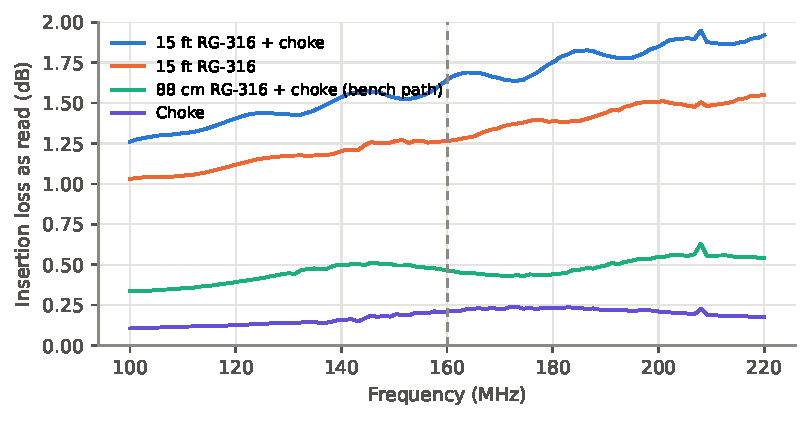
\includegraphics[width=0.85\linewidth]{figures/fig6_vna.pdf}
\caption{Insertion loss as read, 100--220~MHz. The dashed line marks 160~MHz.}
\label{fig:vna}
\end{figure}

\subsection{Receiver calibration}
\label{sec:bench}

The measurement checks out on three counts. Both receivers respond linearly: 10~dB more tone gives
9.9--10.1~dB more reading from $-120$ to $-90$~dBm (Figure~\ref{fig:linearity}). The two Mini runs
agree within 0.05~dB on every tone step and 0.1~dB on the load. With the generator connected and
its output off, both receivers read within 0.1~dB of the 50~$\Omega$ load, so nothing reached them
through the bench's grounding.

\begin{table}[!htbp]
\centering\small
\begin{tabular}{@{}lcc@{}}
\toprule
 & Airspy Mini (gain 21) & Airspy HF+ \\
\midrule
Own noise at the receiver input & $-167.6$\dBmHz & $-166.8$\dBmHz \\
Noise figure, as installed & 6.3--6.4 dB & 7.2 dB \\
Gain $G$, dBm to receiver units & 59.9 dB & 24.1 dB \\
Noise near the tone, rise at $-110$ / $-100$ / $-90$~dBm & +0.4 / +4.8 / +14.0 dB & $<$0.2 dB at all levels \\
Noise across the whole channel, rise at $-90$~dBm & +7.7 to +8.1 dB & $<$0.2 dB \\
\bottomrule
\end{tabular}
\caption{Receiver calibration, 18 November 2026. Both noise figures include whatever the drone's
powered electronics added through the USB connection with the motors off.}
\label{tab:bench}
\end{table}

\begin{figure}[!htbp]
\centering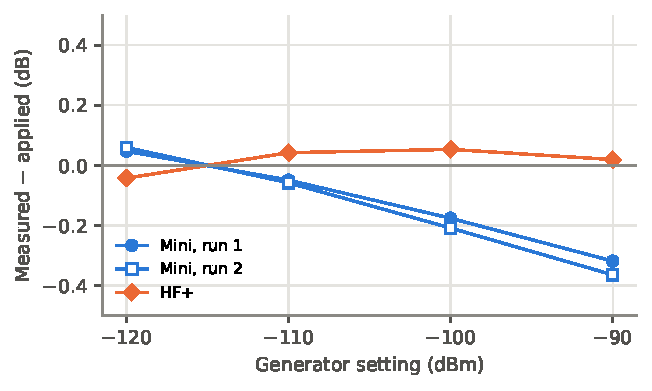
\includegraphics[width=0.6\linewidth]{figures/fig4_linearity.pdf}
\caption{Deviation of the measured tone from the applied level after calibration. Both receivers stay
within 0.4~dB over 30~dB.}
\label{fig:linearity}
\end{figure}

\begin{figure}[!htbp]
\centering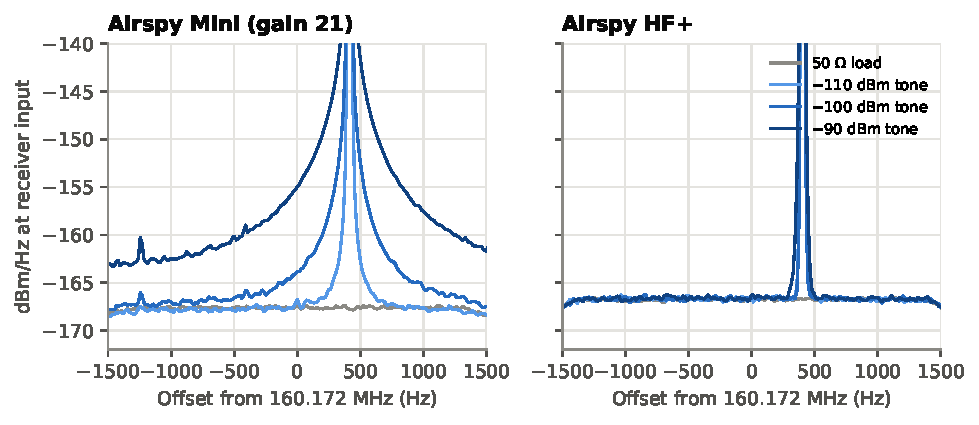
\includegraphics[width=\linewidth]{figures/fig5_desense.pdf}
\caption{Spectrum near the tone at each level, referred to the receiver input. The Mini's noise rises
around a strong tone; the HF+'s does not. The generator was the same for both, so the effect is the
Mini's.}
\label{fig:desense}
\end{figure}

The Mini is about 0.8~dB more sensitive than the HF+ as installed. The HF+'s advantage is its
handling of strong signals: around a tone of $-100$~dBm the Mini's noise rose 5~dB, and around
$-90$~dBm, 14~dB, while the HF+'s did not move. In the field that matters when the drone is close to
a strong tag, where the signal-strength peak is picked, and when a strong interferer sits near the
tag's frequency.

\subsection{Flights}
\label{sec:flights}

\begin{table}[!htbp]
\centering\small
\begin{tabular}{@{}llccc@{}}
\toprule
Flight & Configuration & Ground, motors off & Steady flight & Flight, above own noise \\
\midrule
F2 & Choke + 15 ft coax & $-167.3$ & $-163.5$ & +3.3 dB \\
F3 & Choke + 15 ft coax & $-166.8$ & $-163.5$ & +3.3 dB \\
F7 & Choke, no extension & $-165.3$ & $-161.5$ & +5.2 dB \\
F5 & No choke, 15 ft coax & $-165.9$ & $-161.8$ & +5.0 dB \\
F6 & No choke, no extension & $-155.2$ & $-156.6$ & +10.2 dB \\
P2 & Ponui, old setup & $-161.6$ & $-145.5$ & +22.1 dB \\
P3 & Ponui, old setup & $-162.5$ & $-145.1$ & +22.5 dB \\
\bottomrule
\end{tabular}
\caption{Noise at the receiver input in dBm/Hz. ``Above own noise'' compares with each receiver's
50~$\Omega$ reading (Table~\ref{tab:bench}).}
\label{tab:flights}
\end{table}

\begin{figure}[p]
\centering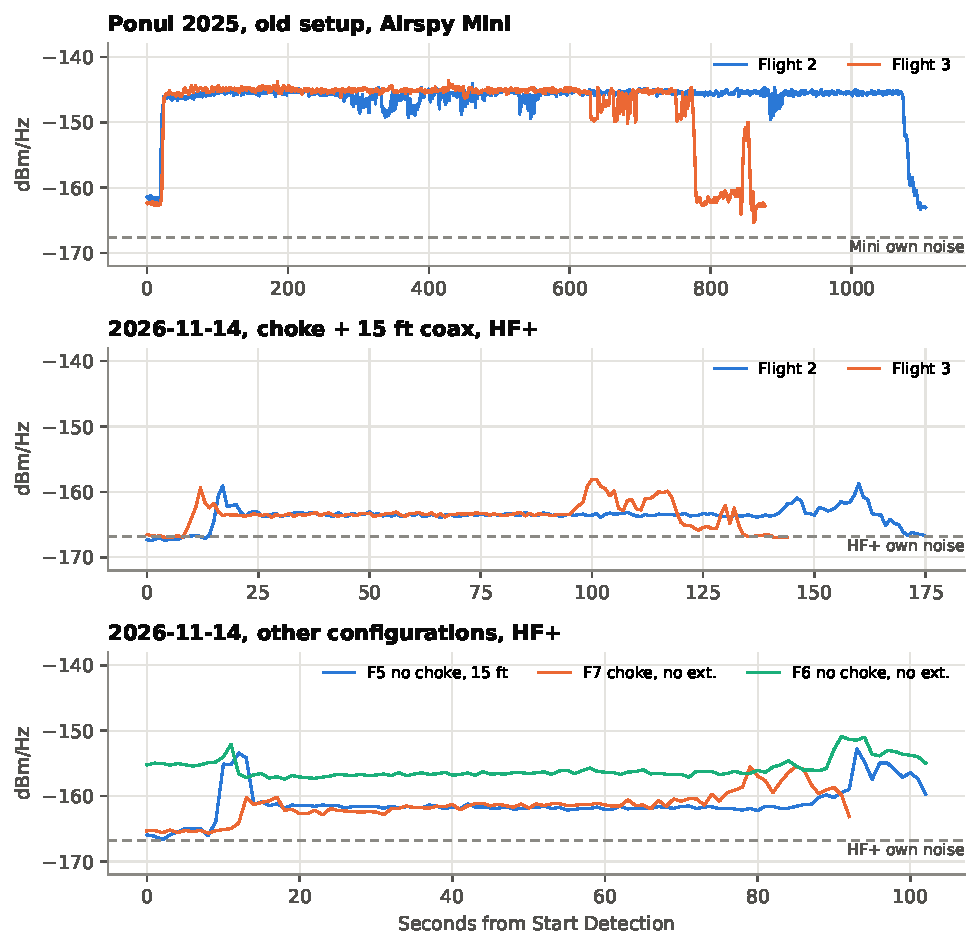
\includegraphics[width=\linewidth]{figures/fig2_timelines.pdf}
\caption{Noise floor second by second. The rise near the start of each 2026 flight is takeoff; the
excursions near the end are probably landing (no telemetry yet). Note the different time scales:
the Ponui flights were much longer.}
\label{fig:timelines}
\end{figure}

\begin{itemize}
\item \textbf{Choke and 15~ft coax together are best} in every stage of flight (F2, F3).
\item \textbf{The choke matters most when the antenna is close to the drone.} Without the extension,
adding the choke (F6 to F7) lowered the noise about 10~dB on the ground and 5~dB in flight. With the
15~ft coax (F5 to F2/F3) it was worth about 1.7~dB in flight, though those flights also flew at
different heights.
\item \textbf{The 15~ft coax matters most without the choke.} Without the choke, the extension
(F6 to F5) bought about 10.7~dB on the ground and 5~dB in flight.
\item \textbf{F6's noise is there before the motors turn.} With no choke and the antenna close,
the noise was 11.6~dB above the receiver's own on the ground and did not rise in flight. The
drone's electronics, not its motors, set it.
\item \textbf{Takeoff and landing add short bursts} of 3--8~dB above the steady level.
\item \textbf{Narrow interference tones remain}, up to 6--10~dB above the floor in some
configurations (Figure~\ref{fig:spectra}), at roughly $-1450$, $-1200$, $-730$, $-380$, $+250$,
$+960$ and $+1270$~Hz from 160.172~MHz. Ponui's in-flight noise was flat across the channel.
\item \textbf{Three false detections occurred in F3}, all at the edge of the detector's channel
($+1920$~Hz), during a 5~dB rise in the noise about 94~s into the flight.
\end{itemize}

\begin{figure}[!htbp]
\centering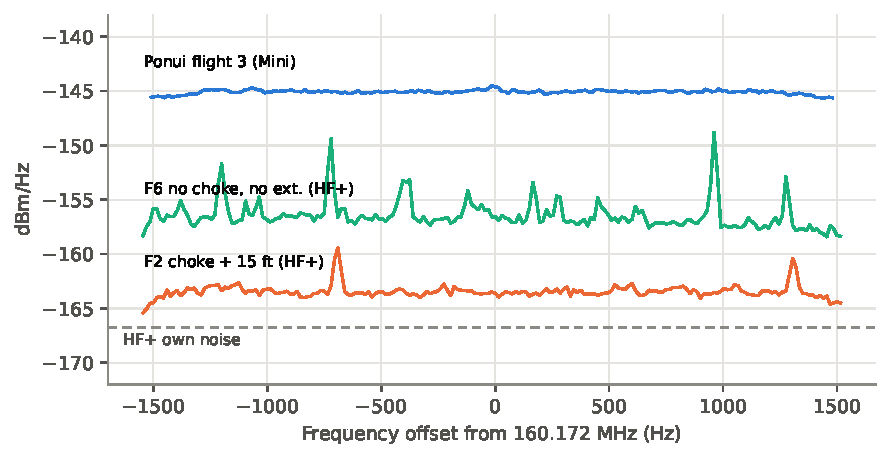
\includegraphics[width=\linewidth]{figures/fig3_spectra.pdf}
\caption{Spectrum in steady flight across the detector's channel.}
\label{fig:spectra}
\end{figure}

\subsection{How much of what remains is the drone}
\label{sec:budget}

\begin{figure}[!htbp]
\centering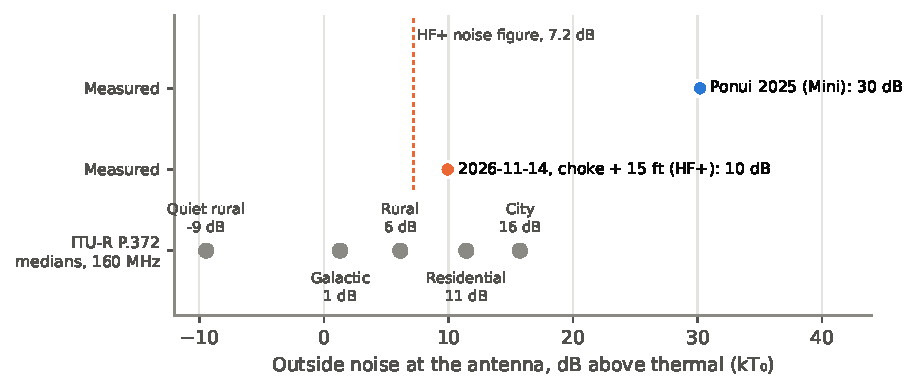
\includegraphics[width=0.9\linewidth]{figures/fig7_budget.pdf}
\caption{Outside noise at the antenna inferred from the flights (Section~\ref{sec:budgetmethod},
feed loss 1.8~dB now and an assumed 1.4~dB at Ponui), against ITU-R P.372 median values at
160~MHz.}
\label{fig:budget}
\end{figure}

On the ground with the motors off, the 14 November noise sat at the receiver's own level. In flight it
rose 3.3~dB. By the noise-addition relation of Section~\ref{sec:budgetmethod}, that rise means about
10~dB of outside noise above $kT_0$ at the antenna: inside the range of ordinary rural to residential
background noise (Figure~\ref{fig:budget}). The 2026 in-flight noise is therefore consistent with the
drone itself adding little or nothing measurable.

This comparison has a known weakness, raised by Michael Shafer: \textbf{on the ground the antenna lies
on the soil}, detuned and at no height, so it delivers little outside noise. The ground reading is
therefore not ``everything but the motors''; the rise into flight combines the motors with the antenna
starting to work. The planned mast test (Section~\ref{sec:next}) measures the background with the
antenna working and the drone off, and will separate the two. \draftnote{Update when the mast test is
done.}

At Ponui the inferred outside noise was about 30~dB above $kT_0$, far above any background level for
a quiet island. That noise was the drone.

\section{Caveats}
\begin{itemize}
\item \textbf{Different sites.} Ponui (rural New Zealand) and the 14 November site (semi-rural
Arizona) have different background noise. The 18~dB improvement includes that difference.
\item \textbf{Mini gain.} Ponui ran the Mini at gain 20; the calibration used 21. Likely 1--2~dB on
the Ponui values.
\item \textbf{Flight stages without telemetry.} Ground, takeoff, steady flight and landing were read
from the noise and the notes. Heights also differed between configurations (170~ft and 50~ft).
\item \textbf{As-installed noise figures.} Both include anything the drone's electronics add through
USB with the motors off.
\item \textbf{Absolute accuracy.} The generator's level and the 0.6~dB path loss are each good to a
few tenths of a decibel. They affect both receivers equally, so the comparison between receivers is
tighter than the absolute numbers.
\end{itemize}

\section{Planned tests}
\label{sec:next}
\begin{enumerate}
\item \textbf{Same-day flights with each receiver}, alternating HF+, Mini, HF+, in the choke + 15~ft
configuration and the 14 November flight profile. Tests whether the Mini picks up out-of-band
signals that the HF+'s front-end filtering rejects --- something the bench could not test, because
the generator came in on a cable rather than through an antenna.
\item \textbf{Background reference}: the antenna raised on a mast with the same coax and choke, the
receiver and Pi on a separate battery, and the drone off and away. Then the same with the drone
powered at the mast's base, motors off.
\item \textbf{A strong-signal pass} with each receiver toward a Tabor LS3081P generator sending tag-like
pulses (20~ms every 1.333~s) from a fixed position, to test the Mini's desensitisation in flight.
\item \textbf{PX4 flight logs} for all flights, to replace the inferred flight stages with altitude and
throttle.
\end{enumerate}

\appendix
\section{Data and scripts}
\begin{itemize}
\item Raw recordings and notes, in OneDrive \texttt{FLIGHT\_TESTING\_DATA/}:
  \texttt{2025-03-23-Ponui-Day8-Sun}; \texttt{2026-11-14-Rail-X\_Ranch\_Road};
  \texttt{2026-11-18-Office\_HF\_v\_Mini\_Testing}.
\item Per-test notes, VNA files and derived data: \texttt{hardware/noise-reduction/} in the UAV-RT hub
repository.
\item Scripts: \texttt{tools/noise\_floor.py}, \texttt{tools/bench\_calibration.py},
\texttt{tools/noise\_report\_data.py} (rebuilds all derived data), and
\texttt{hardware/noise-reduction/report/make\_figures.py}.
\end{itemize}

\end{document}
